% Metódy inžinierskej práce

\documentclass[10pt,twoside,slovak,a4paper]{article}

\usepackage[slovak]{babel}
%\usepackage[T1]{fontenc}
\usepackage[IL2]{fontenc} % lepšia sadzba písmena Ľ než v T1
\usepackage[utf8]{inputenc}
\usepackage{graphicx}
\usepackage{url} % príkaz \url na formátovanie URL
\usepackage{hyperref} % odkazy v texte budú aktívne (pri niektorých triedach dokumentov spôsobuje posun textu)

\usepackage{cite}
\usepackage{times}
\usepackage{float}

\pagestyle{headings}

\title{Použitie hier a VR pri rehabilitácii\thanks{Semestrálny projekt v predmete Metódy inžinierskej práce, ak. rok 2022/23, vedenie: Ing. Igor Stupavský}} % meno a priezvisko vyučujúceho na cvičeniach

\author{Pavol Čížik\\[2pt]
	{\small Slovenská technická univerzita v Bratislave}\\
	{\small Fakulta informatiky a informačných technológií}\\
	{\small \texttt{xcizik@stuba.sk}}
	}

\date{\small 30. september 2022} 



\begin{document}

\maketitle

\begin{abstract}
Vo svojom článku by som sa chcel venovať téme použitie virtuálnej realita a gamifikácie pri rehabilitáciach. Takéto rehabilitácie by sa mohli použiť po zlomeninách alebo u pacientov po mŕtvici. Pretože medzi následky mŕtvice patrí nemožnosť normálnych kontrolovaných pohybov a problémy s hmatom a jemnou motorikou. 

V článku by som sa chcel zamerať na výhody a nevýhody, ktoré by takáto liečba priniesla. Pozrieť sa na ceny virtuálnych realít. A či by bolo možné rehabilitovať aj doma. 

Hry a virtuálna realita by mohli pacientov viacej motivovať do cvičenie čo by mohlo mať za dôsledok rýchlejšie zotavenie. Preto si myslím že táto téma má veľký význam a v budúcnosti by mohli hry a virtuálna realita výrazne pomôcť pri rehabilitáciach.
\end{abstract}



\section{Úvod}

V posledných rokoch sa poožitie VR a hier rozšírilo do mnohých oblastí života. V článku sa zameriavam presnejšie na použitie v zdravotníctve. Specifickejšie použitie hier a VR pri rehabilitáciach, či už u pacientov po mŕtvici ale aj pri bežných úrazoch. 

Napríklad sa zameriavam na VR nástroj Leap motion. Ďalším nástrojom použitím v medicíne je  SilverTune. Ktorá pomáha pacientom po mŕtvici. V článku sa zameriavam ale aj na iné nástroje ktoré sú použité napríklad aj pri rehabilitácii členku. 

Samozrejme všetko má svoje výhody ale aj nevýhody preto sú v článku zhrnuté aj výhody a nevýhody, ktoré použitie týchto zariadení so sebou prináša.

\newpage

\section{Použitie v praxi}


\subsection{SilverTune}\cite{9483850}
SilverTune je nástroj, ktorý je výsledkom výskumu, ktorého hlavným cielom bolo vytvoriť multi-senzorový hudobný nástroj. Výskum sa zameriaval na použitie tohto nástorje pri rehabilitácií starších pacientov po mŕtvici v Singapure.
\newline

\begin{tabular}{ |p{3cm}|p{3cm}| }
\hline
\multicolumn{2}{|c|}{Charakteristika zúčastnených} \\
\hline
Počet zúčastnených & 11 \\
\hline
Priemerný vek & 69 \\
\hline
Mužov & 7 \\
\hline
Žien & 4 \\
\hline
Čas od mŕtvice & 12 až 72 mesiacov \\
\hline
\end{tabular}
\newline
\newline
\newline
SilverTune je ako hudobný nástroj, ktorý poskytuje šesť typov hudobných zvukov a herných interakcií, aby uspokojil rôzne preferencie pacientov a terapeutické požiadavky na pohyb. 

SilverTune môže tiež zaznamenávať údaje, analyzovať výkon v reálnom čase a poskytovať spätnú väzbu pacientom aj terapeutom.

Mobilná aplikácia SilverTune bola vyvinutá ako sprievodná pre muzikoterapiu SilverTune. Aplikácia zaznamenáva profil používateľa a údaje zadané zo SilverTune pre budúcu analýzu terapeutom. 

Na hranie pomocou zariadenia SilverTune boli vyvinuté dve hry. Prvou je dostihová hra, v ktorej sa kôň pohybuje po dostihovej dráhe. Druhou je stolnotenisová hra\ref{fig:SilverTune Stolný tennis}, v ktorej sa loptička na stolný tenis musí podávať cez sieť, aby sa získali body. Dostihová hra uľahčovala ohýbanie a predlžovanie ramien, zatiaľ čo stolnotenisová hra uľahčovala horizontálny únos a addukciu ramena.

\begin{figure}
    \centering
    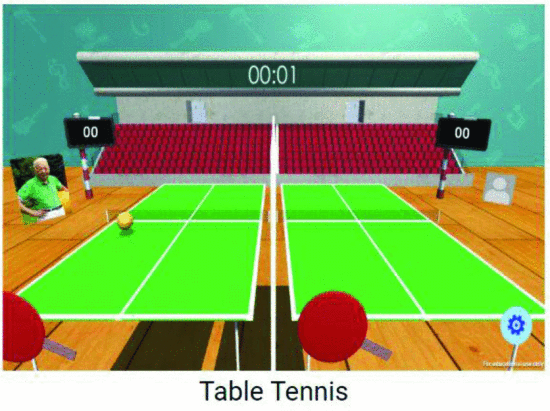
\includegraphics[width = 0.5\textwidth]{obrazky/table_tennnis.png}
    \caption{Stolný tennis}
    \label{fig:SilverTune Stolný tennis}
\end{figure}


\subsection{Leap motion}\cite{7926560}
Leap motion dostal veľa pozornosti v posledných pár rokoch z dôvodu jeho nemeratelného množstva použití ako napríklad robotika, vzdelávanie, medicína atď. Hlavnou myšlienkou gamifikácie rehabilitácie je pomôcť rozvíjať svalový tonus, zefektívniť rehabilitáciu a motivovať pacientov.

Ukázalo sa, že VR a hry sú prospešné pri zlepšovaní funkcie horných končatín, ak sa používajú ako doplnok k bežnej starostlivosti alebo v porovnaní s konvenčnou terapiou.

Hra bola vyvinutá  pomocou Unity 3D a volá sa Escape game\ref{fig:LeapMotion escape game}. Hra má rôzne možnosti, úlohy a cvičenia súvisiace s 3D chytaním, ukazovaním, zdvíhaním, hádzaním a ďalšími cvičeniami na rehabilitáciu rúk. Hlavnou súčasťou tejto VR rehabilitácie je Leap Motion, ktorý sleduje ruky. 

Všetky predmety a štruktúry hry boli vytvorené v Autodesk 3D Max a Cinema 4D, potom importované do prostredia Unity.

\begin{figure}
    \centering
    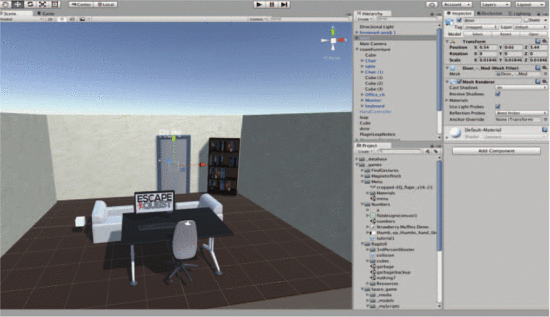
\includegraphics[width = 0.5\textwidth]{obrazky/Escape game.png}
    \caption{Escape game}
    \label{fig:LeapMotion escape game}
\end{figure}

\subsection{Myo armband}\cite{7088817}
Systém na rehabilitácie rúk, inšpirovaný videohernými zariadeniami. Tento systém sa skladá z Myo band a robotickej rukavice. Myo band je nositeľné zariadenie v hodnote ~200 eur.\ref{fig:Myoband pohyby}

Zariadenie poskytuje dva druhy údajov, priestorové a gestové. 
Priestorové údaje informujú o orientácii a pohybe ramena používateľa, zatiaľ čo gestové údaje informujú o tom, čo používateľ robí rukou. Všetky údaje sa komunikujú cez Bluetooth s Unity3D. Tatktiež sú použité dotykové ploch  na detekciu úplne otvorenej/zatvorenej ruky.

V Unity 3D bola vytvorená hra na tréning ruky, v ktorej musí používateľ chytiť, držať a prepravovaťa kocku v niekoľkých čoraz náročnejších úrovniach. V hre hráč vidí virtuálne ruky/ramená, ktoré replikujú pohyby používateľa, vďaka tomu sa použvateľ cíti viacej ponorený do hry. 

V súčasnosti hra funguje nasledovne: používateľ nosí Myo band na zdravom predlaktí a vykonáva požadované pohyby, ktoré sa premietajú do pohybu virtuálnej ruky.
Pohyby rúk sa potom replikujú  do pohybu robotickej rukavice, ktorú používateľ nosí na rehabilitovanej ruke.\ref{fig:Diagram}

\begin{figure}[H]
    \centering
    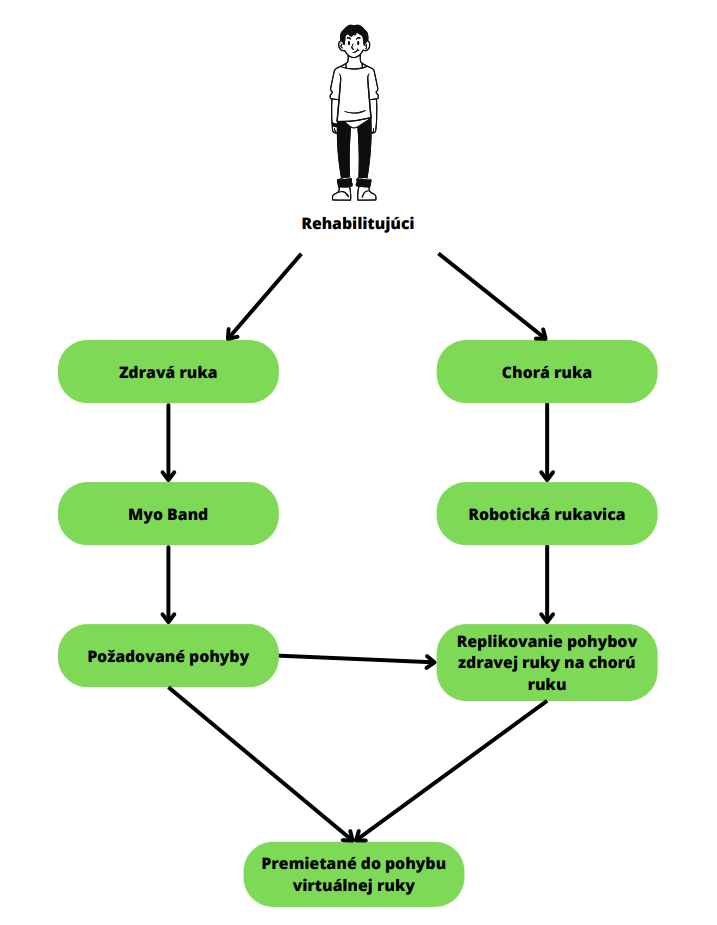
\includegraphics[width = 0.5\textwidth]{obrazky/Diagram.png}
    \caption{Diagram}
    \label{fig:Diagram}
\end{figure}
 
Systém bol doteraz testovaný iba na zdravých jedincoch, ale plánujú sa aj testy s pacientami po mozgovej príhode. Preto je tažké jednoznačne povedať či je tento spôsob rehabilitácie účinný a  sú stále potrebné daľšie testy a štúdie na preukázanie benifitov pre pacientov.

\begin{figure}[H]
    \centering
    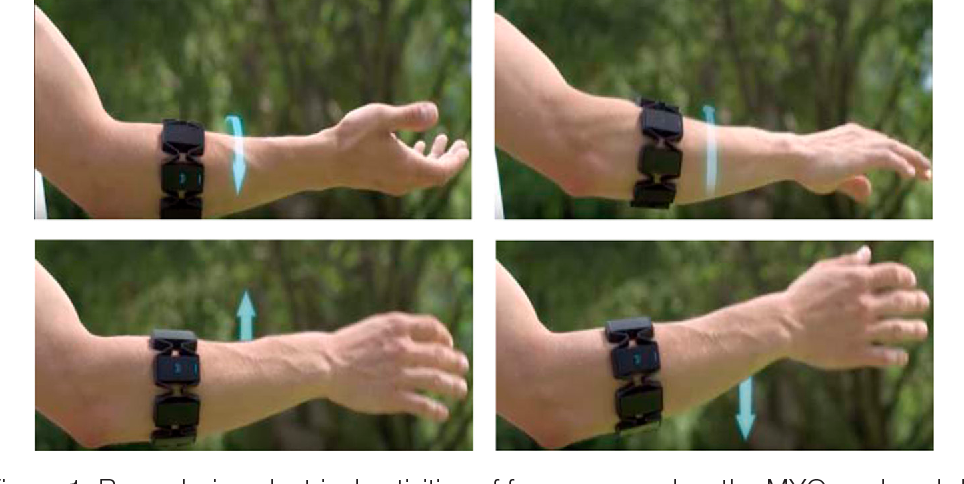
\includegraphics[width = 0.5\textwidth]{obrazky/Myoband.png}
    \caption{Myoband}
    \label{fig:Myoband pohyby}
\end{figure}

\subsection{PhyRe UP!}\cite{9564051}
PhyRe UP! je nový diaľkový rehabilitačný systém, ktorý využíva zmiešanú realitu a gamifikačné techniky\ref{fig:phyre}. PhyRe Up! bol navrhnutý pre pacientov s mozgovou príhodou, aby vykonávali terapeutické cvičenia doma, s veľkou presnosťou a s potenciálnym dohľadom lekárov. 

Cieľom systému je zvýšiť motiváciu pacienta, ako aj udržať kvalitu a výkon pri cvičení, podobne ako pri účasti na osobných stretnutiach s terapeutmi. Základná architektúra kombinuje deklaratívne, procedurálne a podmienené znalosti na riadenie rehabilitačného procesu, ktorý ponúka flexibilitu a škálovateľnosť na zlepšenie schopností navrhovaného systému. 

Experimentálne výsledky poukazujú na to, ako kombinácia zmiešanej reality a gamifikácie významne ovplyvňuje presnosť rehabilitačných cvičení, ktoré predtým definovali terapeuti. Najmä vykonané experimenty v prvej validačnej fáze PhyRe Up! ukazujú, že vizuálna spätná väzba výrazne znižuje medzikroky potrebné na dokončenie cvičenia. Presnosť, s akou pacient vykonáva hodnotené cvičenie prvýkrát, je väčšia ako pri použití tradičných rehabilitačných techník.

\begin{figure}[H]
    \centering
    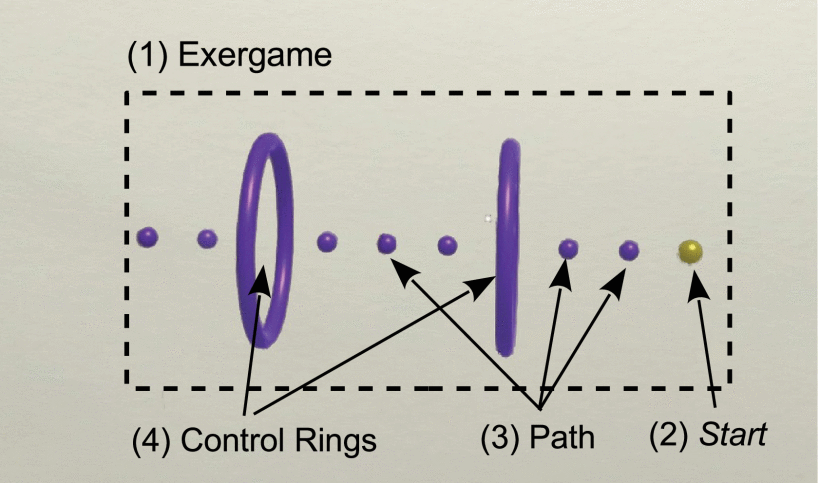
\includegraphics[width = 0.5\textwidth]{obrazky/PhyRe UP!.png}
    \caption{Cvičenie s PhyRe UP!}
    \label{fig:phyre}
\end{figure}

\subsection{Nintendo Wii}\cite{8940302}
Nintendo Wii, pôvodne navrhnuté na zábavné účely, používalo sa v mnohých terapeutických výskumoch. Nintendo Wii je virtuálny systém, ktorý sa používa pri rehabilitácii po celom svete. Táto technológia priťahuje veľkú pozornosť vďaka svojim dostupným nákladom a možnosti použitia ako domáca terapia. Športové hry Wii sú opakujúce sa, špecifické a vedú k lepším terapeutickým výsledkom.

Tréningový program pozostával z 30 minút konvenčnej rehabilitácie, po ktorej nasleduje 30 minút hernej terapie Nintendo Wii 2 dni v týždni, počas 5 týždňov. Herný systém Nintendo Wii vyžaduje aby účastníci používali aktívne pohyby horných končatín na interakciu s virtuálnym prostredím. Každá relácia pozostávala z 35 minút hernej terapie Nintendo Wii s 5 minútami odpočinku. Terapeut bol prítomný na pomoc a kvôli bezpečnosti.

Nintendo Wii poskytuje bezdrôtový ovládač so zabudovanými senzormi zrýchlenia, ktoré detekujú zmeny v pohyboch a zrýchlení. Nintendo Wii bol kalibrovaný pred každým sedením, aby sa zaručilo, že pacient správne používal ovládač postihnutou rukou. U pacientov, ktorí neboli schopní ovládač držať, sa na upevnenie na ruku použil jednoduchý obväz. Boli vybrané dve hry Wii a hrali sa v stoji. 

Terapia založená na hrách vo virtuálnej realite pomocou Nintendo Wii hier v kombinácii s klasickou rehabilitáciou sa ukázala ako účinná pri zotavení hornej končatiny u pacientov po mozgovej príhode. Jednoduchosť, bezpečnosť a nákladová efektívnosť systému virtuálnej reality by mohli podporiť jeho integráciu do rehabilitačných programov.

\subsection{AnkleBot}\cite{7523762}
AnkleBot od IMT\ref{fig:anklebot}, je rehabilitačným mechanizmom pre dolnú časť tela, konkrétne pre členok. Funguje na platforme Ubuntu verzie 5.1 a jej riadiaci algoritmus bol vyvinutý v jazyku C. 

Robot je pripevnený na kolennú ortézu a pripojený k topánke navrhnutej na mieru. Keď človek pohybuje členkom, robot pohybuje chodidlom po naprogramovanej trajektórii v rôznych smeroch v rámci normálneho rozsahu pohybu členku.

\begin{figure}
    \centering
    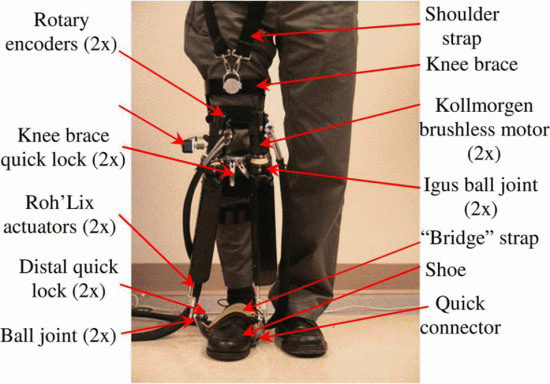
\includegraphics[width = 0.7\textwidth]{obrazky/AnkleBot.png}
    \caption{AnkleBot}
    \label{fig:anklebot}
\end{figure}

\section{Výhody použitia virtuálnej reality pri rehabilitáciach} 

Jednou z hlavných výhod VR a hier je , že rehabilitácie vedia prebiehať na dialku. Táto metóda sa ukázala ako zábavnejšia a viac motivujúca. Motivujúci pre pacientov môže byť aj fakt že ďalší členovia rodiny sa môžu pridať a zdravá súťaživosť je ďalšia motivácia podať čo najlepší výkon. Ďalšou výhodou je že virtuálna realita a hry by mohli odlahčiť nátlak na telecvične a na terapeutov. Jeden terapeut by sa dokázal venovať viacerým pacientom a zároveň telecvične by bole volnejšie pre pacientov pre ktorých rehabilitácia s použitím VR nie je možná. Medzi ďalšie výhody patrí možnosť ukladania údajov vďaka čomu má pacient aj motiváciu v tom že vidí čo už dokázal.



\section{Nevýhody použitia virtuálnej reality pri rehabilitáciach}
Ako všetko aj rehabilitácie s virtuálnou realitou majú výhody aj nevýhody. Medzi nevýhody patrí aj nákladovosť. Tieto zariadenia sú finančne náročné či už na zaobstaranie alebo na údržbu. A zároveň zaobstaranie virtuálnej reality nestačí ak sa nejedná napríklad o Nintendo WII a je potrebné aj zaobstaranie výkonného počítaču. Zároveň nie všetci terapeuti majú dostatočné technické schopnosti aby s týmito zariadeniami vedeli pracovať. Ďalšie doškolovanie by malo za následok ďalšie výdavky.
A zároveň nie všetci pacienty majú na to aby si vedeli nejaké takéto zariadenie zaobstarať. Jedným s riešením by bolo že nemocnice alebo poistovne by vedeli tieto zariadenia požičiavať ale bolo by potrebné zaobstarať dostatočné počty týchto zariadení.


\section{Reakcia na témy z prednášok}
\paragraph{Technológia a ľudia}
Rehebilitácie s použitím virtuálnej reality a hier je ďalším spôsobom ako začleniť technológie do bežného života.Ale ako je to s každou technológoiou je potrebné aby ľudia používajúci tieto technológie mali zručnosti na to aby s ňou dokázali správne pracovať.Pre súčastných terapeutov by sa mohli zaviesť preškolenia a budúca generácia terapeutov by sa mohla už na škole učiť ako pracovať s týmito technológiami. Použitie virtuálnej reality pri rehabilitácii je skvelý spôsob ako začleniť IT sektor do medicíny a životov ľudí.

\paragraph{Spoločenské súvislosti}
Rehabilitácie pomáhajú luďom doliečiť zranenia a po vážnych zraneniach a mŕtvici obnoviť správnu funkčnosť končatín. Rehabilitácie pomáhajú týmto ľudom vrátiť sa k bežnému životu a znova sa začleniť spoločensky a aj pracovne a žiť bežný život ako pred zranením. Virtuálna realita a hry by mohli tento proces urýchliť a zefektívniť. Alebo dokonca pomôcť luďom ktorým bežná rehabilitácia nedokázala dostatočne pomôcť k správnej funkcii ako pred zranením.

\paragraph{Udržatelnosť a etika}
Je tažké povedať či výroba toľkých zariadení VR je do budúcnosti udržatelné ale jednou s možností ako spraviť rehabilitácie s VR udržatelnejšie je vyradené kusy ktoré nie sú poškodené a sú plne funkčné by sa mohli darovať na domácu rehabilitáciu ľudom ktorý si kúpu takéhoto zariadenia nemôžu dovoliť. A zároveň domáce rehabilitácie sú voči ľudom ktorý majú problémy s pohybom alebo bývajú ďaleko a nemajú sa ako na rehabilitácie dostať omnoho etickejšie.


\section{Záver} 
Osobne si myslím že virtuálna realita a hry by sa mohli stáť bežnou súčasťou rehabilitácii. Buď by mohli byť kombinované s tradičnou rehabilitáciou alebo ju kompletne nahradiť. 

Osobne si ale myslím že bude eštre potrebných pár rokov aby sa virtuálna realita a hry mohli zaviesť do rehabilitácií. Určite budú ešte potrebné dalšie výskumi aby sa zistilo ako najlepšie a najefektívnejšie túto technológiu využiť pri rehabilitáciach a pri akých zraneniach je efektívne použitelná. 

Je to skvelí spôsob ako zapojiť IT sektor do medicíny, ako prispôsobiť rehabilitácie individuálnym potrebám každého pacienta, pretože virtuálna realita a hry sú veľmi flexibilné a multifunkčné.  Podľa môjho názoru zatiaľ neexistuje potrebné množstvo hier aby pokrili všetky potreby pacientov a bude potrebný ďalší vývoj hier ktoré budú určené na rehabilitácie. Zároveň celoplošné zavedenie virtuálnej reality ako súčasti rehabilitácie by bolo finačne náročné a zároveň väčšina personálu nemá potrebné zručnosti na ovládanie týchto zariadení. Takže určite budé potrebné ďalšie zaškolenie terapeútov. Určite by pomohlo keby sa budúce generácie terapeútov už na škole učili ako s takýmito technológiami pracovať. 

Myslím že to ešte pár rokov potrvá ale sme na dobrej ceste k tomu aby sa virtuálna realita a hry bežne používali počas rehabilitácii a pomáhali ľudom k rýchlemu a kompletnému zotaveniu.

\bibliography{literatura}
\bibliographystyle{plain} % prípadne alpha, abbrv alebo hociktorý iný
\end{document}
